% ==============================================================================
%  SiliconForge: From Netlist to Phase Noise
%  A Pedagogical Journey Through EDA Stack
% ==============================================================================
\documentclass[aspectratio=169, 11pt]{beamer}
\usetheme{Madrid}
\usecolortheme{default}
\setbeamertemplate{navigation symbols}{}
\setbeamertemplate{footline}[frame number]

\usepackage{tikz}
\usetikzlibrary{arrows.meta, shapes.geometric, positioning, calc, decorations.pathreplacing, patterns}
\usepackage[american]{circuitikz}
\usepackage{pgfplots}
\pgfplotsset{compat=1.18}
\usepackage{amsmath, amssymb}
\usepackage{booktabs}
\usepackage{listings}
\usepackage{xcolor}
\usepackage{siunitx}
\usepackage{graphicx}
\usepackage{adjustbox}
\usepackage{array}

\definecolor{myblue}{RGB}{31,78,121}
\definecolor{myorange}{RGB}{214,110,20}
\definecolor{mygreen}{RGB}{20,125,60}
\definecolor{myred}{RGB}{180,40,40}
\definecolor{lightblue}{RGB}{200,220,240}
\definecolor{lightgray}{RGB}{245,245,245}

\setbeamercolor{title}{fg=white,bg=myblue}
\setbeamercolor{frametitle}{fg=white,bg=myblue}
\setbeamercolor{structure}{fg=myblue}
\setbeamercolor{block title}{fg=white,bg=myblue}
\setbeamercolor{block body}{bg=lightblue}

\lstdefinestyle{pythonstyle}{
    backgroundcolor=\color{lightgray},
    commentstyle=\color{mygreen},
    keywordstyle=\color{myblue},
    numberstyle=\tiny\color{gray},
    stringstyle=\color{myorange},
    basicstyle=\ttfamily\scriptsize,
    breakatwhitespace=false,
    breaklines=true,
    captionpos=b,
    keepspaces=true,
    numbers=left,
    numbersep=5pt,
    showspaces=false,
    showstringspaces=false,
    showtabs=false,
    tabsize=2,
    language=Python,
    columns=fullflexible,
}
\lstset{style=pythonstyle}

\title[SiliconForge]{From Netlist to Phase Noise}
\subtitle{A Pedagogical Journey Through the SiliconForge EDA Stack}
\author{Hosakota Ganesh Kumara}
\date{August 2026}

\begin{document}

\begin{frame}
\titlepage
\end{frame}

% ==============================================================================
% PART 1: THE PHYSICAL PROBLEM (Slides 1-8)
% ==============================================================================

\section{Part 1: Why Oscillators?}

\begin{frame}{1. The World Runs on Clocks}
    \textbf{Every digital system needs a clock:}
    \begin{itemize}
        \item Microprocessors: GHz clocks drive instruction execution
        \item Radios: LO clocks mix signals up and down
        \item Sensors: clocks timestamp measurements
        \item Communication: clocks synchronize data transfer
    \end{itemize}

    \vspace{0.5em}
    \begin{block}{The Ideal vs Reality}
        \textbf{Ideal:} $v(t) = A \cos(2\pi f_0 t)$ — a perfect sinusoid at exactly $f_0$.

        \textbf{Reality:} $v(t) = A(t)\cos(2\pi f_0 t + \phi(t))$ — amplitude and phase wander.
    \end{block}
\end{frame}

\begin{frame}{2. What Is Phase Noise?}
    \textbf{Phase noise $\mathcal{L}(f)$ measures how much power leaks into adjacent frequencies.}

    \vspace{0.5em}
    \begin{center}
        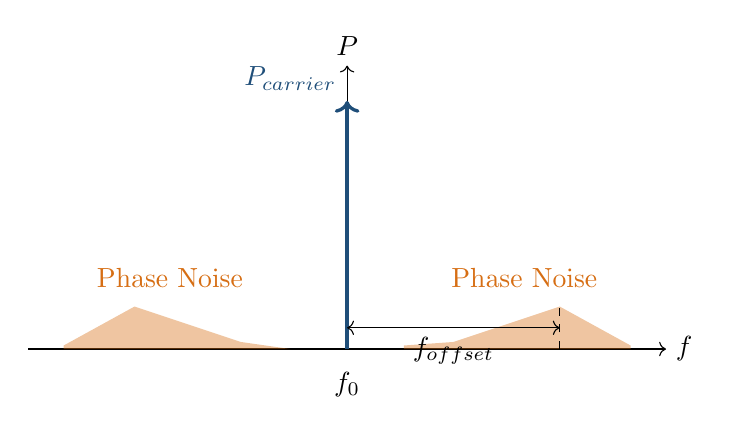
\begin{tikzpicture}[scale=0.9]
            \draw[->] (-4.5,0) -- (4.5,0) node[right] {$f$};
            \draw[->] (0,0) -- (0,4) node[above] {$P$};
            % Carrier
            \draw[->, very thick, myblue] (0,0) -- (0,3.5) node[above left] {$P_{carrier}$};
            % Noise sidebands
            \fill[myorange, opacity=0.4] (-4,0) -- (-4,0.05) -- (-3,0.6) -- (-1.5,0.1) -- (-0.8,0) -- cycle;
            \fill[myorange, opacity=0.4] (0.8,0) -- (0.8,0.05) -- (1.5,0.1) -- (3,0.6) -- (4,0.05) -- (4,0) -- cycle;
            % Annotation
            \draw[<->] (0,0.3) -- (3,0.3) node[midway, below] {$f_{offset}$};
            \draw[dashed] (3,0) -- (3,0.7);
            \node at (0,-0.5) {$f_0$};
            \node[myorange] at (-2.5,1) {Phase Noise};
            \node[myorange] at (2.5,1) {Phase Noise};
        \end{tikzpicture}
    \end{center}

    \vspace{0.3em}
    \[ \mathcal{L}(f_{offset}) = 10\log_{10}\left(\frac{P_{noise}(f_0 + f_{offset})\ \text{in 1 Hz}}{P_{carrier}}\right) \text{ dBc/Hz} \]
\end{frame}

\begin{frame}{3. Why Does Phase Noise Matter?}
    \textbf{Real consequences of phase noise:}

    \vspace{0.5em}
    \begin{columns}[T]
        \begin{column}{0.48\textwidth}
            \textbf{Radar:}
            \begin{itemize}
                \item A ghost target appears next to the real one
                \item Weak signals buried in noise sidebands
            \end{itemize}
            \vspace{0.3em}
            \textbf{Communications:}
            \begin{itemize}
                \item Adjacent channel interference
                \item Increased bit error rate
            \end{itemize}
        \end{column}
        \begin{column}{0.48\textwidth}
            \textbf{Digital:}
            \begin{itemize}
                \item Timing jitter, setup/hold violations
                \item Reduced maximum clock frequency
            \end{itemize}
            \vspace{0.3em}
            \textbf{Sensors:}
            \begin{itemize}
                \item Reduced sensitivity
                \item False detections
            \end{itemize}
        \end{column}
    \end{columns}

    \vspace{0.5em}
    \textcolor{myred}{\textbf{Goal: Predict phase noise BEFORE fabricating silicon.}}
\end{frame}

\begin{frame}{4. A Concrete Example: 30 GHz VCO}
    \textbf{Design target:} 30 GHz LC oscillator in IHP SG13G2 (130nm BiCMOS)

    \vspace{0.5em}
    \begin{columns}[T]
        \begin{column}{0.48\textwidth}
            \textbf{Circuit:}
            \begin{itemize}
                \item Cross-coupled HBT pair
                \item LC tank: $L = 53$ pH, $C = 40$ fF
                \item Tail current: $I_{tail} = 4$ mA
                \item $V_{DD} = 1.2$ V
            \end{itemize}
        \end{column}
        \begin{column}{0.48\textwidth}
            \textbf{Target specs:}
            \begin{itemize}
                \item $f_0 \approx 30$ GHz
                \item $V_{PP} > 0.5$ V
                \item $\mathcal{L}(1\text{MHz}) < -110$ dBc/Hz
                \item Power $< 10$ mW
            \end{itemize}
        \end{column}
    \end{columns}

    \vspace{0.5em}
    \textbf{How do we verify this before fabrication?}
\end{frame}

\begin{frame}{5. The EDA Flow: From Physics to Numbers}
    \textbf{The complete stack:}

    \vspace{0.5em}
    \begin{center}
        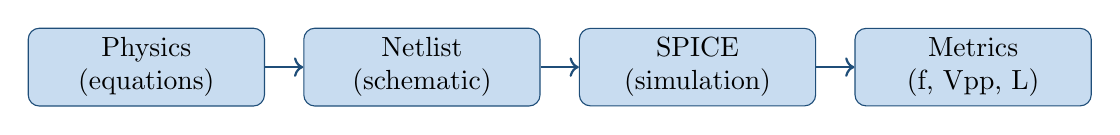
\begin{tikzpicture}[
            box/.style={draw=myblue, fill=lightblue, rounded corners, minimum width=3cm, minimum height=0.8cm, align=center},
            arr/.style={->, thick, myblue}
        ]
            \node[box] (p1) at (0,0) {Physics\\(equations)};
            \node[box] (p2) at (3.5,0) {Netlist\\(schematic)};
            \node[box] (p3) at (7,0) {SPICE\\(simulation)};
            \node[box] (p4) at (10.5,0) {Metrics\\(f, Vpp, L)};

            \draw[arr] (p1) -- (p2);
            \draw[arr] (p2) -- (p3);
            \draw[arr] (p3) -- (p4);
        \end{tikzpicture}
    \end{center}

    \vspace{0.5em}
    \textbf{Today we'll open every box:}
    \begin{enumerate}
        \item How circuits are described (netlists)
        \item How simulators solve them (SPICE internals)
        \item How we extract metrics (frequency, phase noise, jitter)
        \item How it all runs on a CPU (implementation)
    \end{enumerate}
\end{frame}

\begin{frame}{6. What Is a Netlist?}
    \textbf{A netlist is a textual description of a circuit:}

    \vspace{0.5em}
    \begin{columns}[T]
        \begin{column}{0.48\textwidth}
            \textbf{Example: Simple RC}
            \begin{lstlisting}[language=SPICE]
* RC low-pass filter
V1 in 0 PULSE(0 1 0 1n 1n 5n 10n)
R1 in out 1k
C1 out 0 1p
.end
            \end{lstlisting}
        \end{column}
        \begin{column}{0.48\textwidth}
            \textbf{Each line is an element:}
            \begin{itemize}
                \item \texttt{V1}: Voltage source between nodes \texttt{in} and \texttt{0}
                \item \texttt{R1}: Resistor between \texttt{in} and \texttt{out}
                \item \texttt{C1}: Capacitor between \texttt{out} and \texttt{0}
            \end{itemize}
            \vspace{0.3em}
            \textbf{Nodes} are connection points.
            \textbf{Ground} is always node \texttt{0}.
        \end{column}
    \end{columns}
\end{frame}

\begin{frame}{7. Our 30 GHz VCO Netlist (Simplified)}
    \begin{lstlisting}[language=SPICE, basicstyle=\ttfamily\tiny]
* 30 GHz HBT VCO - SiliconForge Benchmark
.lib "/tmp/ihp_sg13g2/libs.tech/ngspice/models/cornerHBT.lib" hbt_typ

VCC vcc_int 0 1.2
* Inductors (53 pH each leg)
L1 vcc_int out_x 53p
L2 vcc_int out_y 53p
* Base capacitors
X_cbase_x out_x 0 cap_cmim l=12.5u w=12.5u
X_cbase_y out_y 0 cap_cmim l=12.5u w=12.5u
* Cross-coupled HBT pair (m=4 for startup)
X1 out_x out_y tail 0 npn13G2l m=4
X2 out_y out_x tail 0 npn13G2l m=4
* Tail current
I_tail tail 0 4m
* Analysis
.tran 0.5p 20n
.end
    \end{lstlisting}
\end{frame}

\begin{frame}{8. From Schematic to Netlist: What Happens?}
    \textbf{The schematic editor writes the netlist for you.}

    \vspace{0.5em}
    \begin{center}
        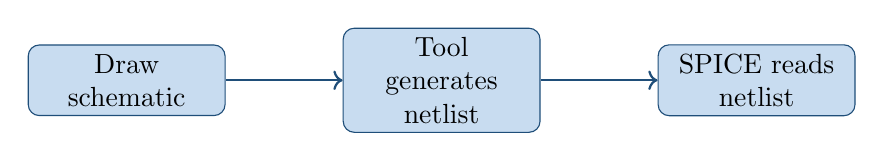
\begin{tikzpicture}[
            box/.style={draw=myblue, fill=lightblue, rounded corners, minimum width=2.5cm, minimum height=0.7cm, align=center},
            arr/.style={->, thick, myblue}
        ]
            \node[box] (s1) at (0,0) {Draw\\schematic};
            \node[box] (s2) at (4,0) {Tool\\generates\\netlist};
            \node[box] (s3) at (8,0) {SPICE reads\\netlist};
            \draw[arr] (s1) -- (s2);
            \draw[arr] (s2) -- (s3);
        \end{tikzpicture}
    \end{center}

    \vspace{0.5em}
    \textbf{Inside the netlist:}
    \begin{itemize}
        \item Each component becomes a line: \texttt{Name nodes model parameters}
        \item Models come from the PDK (Process Design Kit)
        \item Analysis commands tell SPICE what to compute
    \end{itemize}

    \vspace{0.5em}
    \begin{block}{PDK = Process Design Kit}
        Contains transistor models, passive device models, design rules — everything needed to simulate a real silicon process.
    \end{block}
\end{frame}

% ==============================================================================
% PART 2: HOW SPICE WORKS (Slides 9-25)
% ==============================================================================

\section{Part 2: Inside the Simulator}

\begin{frame}{9. What Does SPICE Actually Do?}
    \textbf{SPICE solves the circuit equations:}

    \vspace{0.5em}
    \[ \mathbf{G}(t) \cdot \mathbf{v}(t) + \mathbf{C} \cdot \frac{d\mathbf{v}(t)}{dt} = \mathbf{i}(t) \]

    Where:
    \begin{itemize}
        \item $\mathbf{G}$: Conductance matrix (resistors, linearized transistors)
        \item $\mathbf{C}$: Capacitance matrix (capacitors, transistor parasitics)
        \item $\mathbf{v}(t)$: Node voltages (unknowns we solve for)
        \item $\mathbf{i}(t)$: Current sources (inputs)
    \end{itemize}

    \vspace{0.5em}
    \begin{block}{Key Insight}
        SPICE converts a circuit into a system of differential equations, then solves them step by step in time.
    \end{block}
\end{frame}

\begin{frame}{10. Modified Nodal Analysis (MNA)}
    \textbf{The algorithm SPICE uses to build the equations:}

    \vspace{0.5em}
    \begin{enumerate}
        \item \textbf{Stamp} each element into the $\mathbf{G}$ and $\mathbf{C}$ matrices
        \item \textbf{Apply} voltage source contributions (extra rows/columns)
        \item \textbf{Solve} the linear system at each timestep
        \item \textbf{Update} nonlinear elements (iterate if needed)
    \end{enumerate}

    \vspace{0.5em}
    \begin{block}{Example: Resistor stamp}
        A resistor $R$ between nodes $a$ and $b$ adds to $\mathbf{G}$:
        \[ G_{aa} \mathrel{+}= \frac{1}{R}, \quad G_{ab} \mathrel{-}= \frac{1}{R}, \quad G_{ba} \mathrel{-}= \frac{1}{R}, \quad G_{bb} \mathrel{+}= \frac{1}{R} \]
    \end{block}
\end{frame}

\begin{frame}{11. Transient Analysis: Time-Stepping}
    \textbf{To simulate over time, SPICE uses numerical integration:}

    \vspace{0.5em}
    \begin{columns}[T]
        \begin{column}{0.48\textwidth}
            \textbf{Backward Euler:}
            \[ \frac{dv}{dt} \approx \frac{v(t_n) - v(t_{n-1})}{h} \]
            where $h = t_n - t_{n-1}$ is the timestep.

            \vspace{0.5em}
            \textbf{Trapezoidal Rule:}
            \[ \frac{dv}{dt} \approx \frac{v(t_n) - v(t_{n-1})}{h} + \frac{f(t_n) - f(t_{n-1})}{2} \]
        \end{column}
        \begin{column}{0.48\textwidth}
            \textbf{At each timestep:}
            \begin{enumerate}
                \item Linearize nonlinear elements
                \item Build $\mathbf{G}$ and $\mathbf{C}$ matrices
                \item Solve the linear system
                \item Check convergence (Newton-Raphson)
                \item Advance to next timestep
            \end{enumerate}
        \end{column}
    \end{columns}
\end{frame}

\begin{frame}{12. Newton-Raphson: Solving Nonlinear Equations}
    \textbf{Transistors are nonlinear. SPICE handles this with Newton's method:}

    \vspace{0.5em}
    \[ \mathbf{v}^{(k+1)} = \mathbf{v}^{(k)} - \mathbf{J}^{-1}(\mathbf{v}^{(k)}) \cdot \mathbf{f}(\mathbf{v}^{(k)}) \]

    \vspace{0.5em}
    Where $\mathbf{J}$ is the Jacobian matrix of partial derivatives.

    \begin{center}
        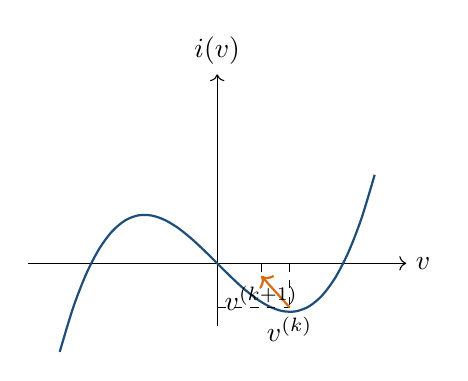
\begin{tikzpicture}[scale=0.8]
            \draw[->] (-3,0) -- (3,0) node[right] {$v$};
            \draw[->] (0,-1) -- (0,3) node[above] {$i(v)$};
            \draw[domain=-2.5:2.5,smooth,variable=\x,myblue,thick] plot ({\x},{\x*\x*\x/4 - \x});
            \draw[dashed] (1.15,0) -- (1.15,-0.7) node[below] {$v^{(k)}$};
            \draw[dashed] (0,-0.7) -- (1.15,-0.7);
            \draw[myorange, thick, ->] (1.15,-0.7) -- (0.7,-0.2);
            \draw[dashed] (0.7,0) -- (0.7,-0.2) node[below] {$v^{(k+1)}$};
        \end{tikzpicture}
    \end{center}
\end{frame}

\begin{frame}{13. SiliconForge's SPICE Interface}
    \textbf{How SiliconForge talks to ngspice:}

    \vspace{0.5em}
    \begin{lstlisting}
def run_ngspice(netlist_path, pdk_root="/tmp"):
    # Convert Windows path to WSL path
    netlist_wsl = _wsl_path(netlist_path)
    
    # Build the shell command
    cmd = f"cd '{workdir}' && export PDK_ROOT='{pdk_root}' " \
          f"&& ngspice -b '{netlist_wsl}' 2>&1"
    
    # Run via WSL subprocess
    result = subprocess.run(
        ["wsl", "bash", "-c", cmd],
        capture_output=True, text=True, timeout=300
    )
    return result.stdout, result.stderr
    \end{lstlisting}
\end{frame}

\begin{frame}{14. Generating Measurement Commands}
    \textbf{SiliconForge generates \texttt{.meas tran} cards:}

    \vspace{0.5em}
    \begin{lstlisting}
def create_meas_netlist(netlist_path, tstop_ns=50.0):
    # Detect output nodes
    out_node = "out_p"
    out_node_n = "out_n"  # differential output

    # Build measurement cards
    meas_lines = [
        f".tran 0.5p {tstop_ns}n",
        f".meas tran t1 WHEN v({out_node})={threshold} RISE=3",
        f".meas tran t2 WHEN v({out_node})={threshold} RISE=5",
        f".meas tran freq PARAM='1/(t2-t1)'",
    ]
    return netlist_with_meas
    \end{lstlisting}
\end{frame}

\begin{frame}{15. Parsing SPICE Output}
    \textbf{Extract frequency from measurement output:}

    \vspace{0.5em}
    \begin{lstlisting}
def extract_frequency_from_meas(output):
    # ngspice prints: "freq = 1.021448e+10"
    match = re.search(r'freq\s*=\s*([eE\d.+-]+)', output)
    if match:
        return float(match.group(1))
    return None
    \end{lstlisting}

    \vspace{0.5em}
    \textbf{For our 30 GHz VCO:}
    \begin{itemize}
        \item ngspice simulates the transient for 20 ns
        \item Extracts frequency from zero-crossing times
        \item Result: $f_0 = 38.18$ GHz
    \end{itemize}
\end{frame}

\begin{frame}{16. Zero-Crossing Frequency Extraction}
    \textbf{How we measure frequency from a waveform:}

    \vspace{0.5em}
    \begin{columns}[T]
        \begin{column}{0.48\textwidth}
            \begin{lstlisting}
def measure_frequency_zero_crossings(time, voltage):
    v_centered = voltage - np.mean(voltage)
    crossings = []
    for i in range(len(v_centered) - 1):
        if v_centered[i] <= 0 and v_centered[i+1] > 0:
            # Linear interpolation for sub-step accuracy
            slope = (v_centered[i+1] - v_centered[i]) / (time[i+1] - time[i])
            t_cross = time[i] + (0 - v_centered[i]) / slope
            crossings.append(t_cross)

    periods = np.diff(crossings)
    return 1.0 / np.mean(periods)
            \end{lstlisting}
        \end{column}
        \begin{column}{0.48\textwidth}
            \begin{center}
                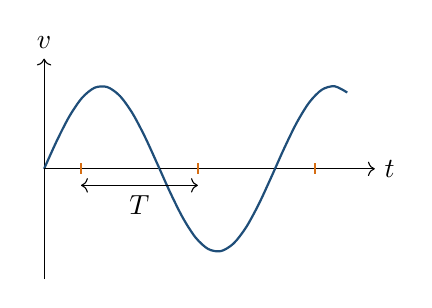
\begin{tikzpicture}[scale=0.7]
                    \draw[->] (0,0) -- (6,0) node[right] {$t$};
                    \draw[->] (0,-2) -- (0,2) node[above] {$v$};
                    \draw[domain=0:5.5,smooth,variable=\x,myblue,thick] plot ({\x},{1.5*sin(deg(1.5*\x))});
                    \draw[dashed] (0,0) -- (6,0);
                    \foreach \x in {0.67, 2.79, 4.91} {
                        \draw[myorange, thick] (\x,0.1) -- (\x,-0.1);
                    }
                    \draw[<->] (0.67,-0.3) -- (2.79,-0.3) node[midway,below] {$T$};
                \end{tikzpicture}
            \end{center}
            \vspace{0.3em}
            \textbf{38 crossings found}\\
            \textbf{Period: 26.19 ps}\\
            \textbf{Freq: 38.18 GHz}
        \end{column}
    \end{columns}
\end{frame}

\begin{frame}{17. The Full Simulation Flow}
    \textbf{From netlist to frequency:}

    \vspace{0.5em}
    \begin{center}
        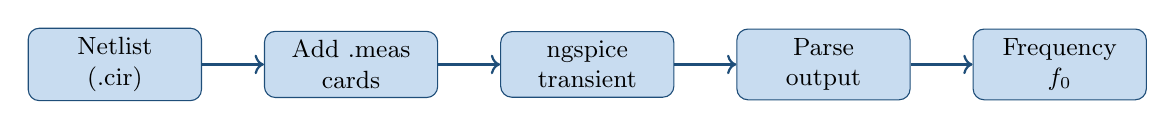
\begin{tikzpicture}[
            box/.style={draw=myblue, fill=lightblue, rounded corners, minimum width=2.2cm, minimum height=0.6cm, align=center, font=\small},
            arr/.style={->, thick, myblue}
        ]
            \node[box] (n1) at (0,0) {Netlist\\(.cir)};
            \node[box] (n2) at (3,0) {Add .meas\\cards};
            \node[box] (n3) at (6,0) {ngspice\\transient};
            \node[box] (n4) at (9,0) {Parse\\output};
            \node[box] (n5) at (12,0) {Frequency\\$f_0$};

            \draw[arr] (n1) -- (n2);
            \draw[arr] (n2) -- (n3);
            \draw[arr] (n3) -- (n4);
            \draw[arr] (n4) -- (n5);
        \end{tikzpicture}
    \end{center}

    \vspace{0.5em}
    \textbf{What ngspice does internally:}
    \begin{enumerate}
        \item Read netlist $\rightarrow$ build MNA matrices
        \item Initialize $\mathbf{v}(0)$ from initial conditions
        \item For each timestep $t_n$:
        \begin{itemize}
            \item Linearize transistors at operating point
            \item Solve $\mathbf{G}\mathbf{v} = \mathbf{i}$ using sparse LU
            \item Newton-Raphson iteration until convergence
        \end{itemize}
        \item Write output to stdout
    \end{enumerate}
\end{frame}

\begin{frame}{18. Why Can't We Just Use .noise Analysis?}
    \textbf{The fundamental problem:}

    \vspace{0.5em}
    \begin{alertblock}{Oscillators Have No DC Operating Point}
        SPICE \texttt{.noise} analysis linearizes around a DC point. But an oscillator's DC point is \textbf{unstable} — that's why it oscillates!
    \end{alertblock}

    \vspace{0.5em}
    \textbf{Commercial tools solve this with:}
    \begin{itemize}
        \item Spectre: PSS (Periodic Steady State) + PNoise
        \item FineSim: Harmonic Balance + HBNoise
    \end{itemize}

    \vspace{0.5em}
    \textbf{SiliconForge's approach:}
    \begin{itemize}
        \item Run a regular transient simulation
        \item Extract the steady-state oscillation
        \item Compute phase noise from the waveform itself
    \end{itemize}
\end{frame}

% ==============================================================================
% PART 3: PHASE NOISE THEORY (Slides 19-35)
% ==============================================================================

\section{Part 3: Phase Noise Theory}

\begin{frame}{19. The Leeson Model: Intuition First}
    \textbf{Leeson (1996) gave an empirical formula:}

    \vspace{0.5em}
    \[ \mathcal{L}(f_{offset}) = 10\log_{10}\left[\frac{2k_B T F}{P_{sig}} \left(1 + \frac{f_0}{2Q f_{offset}}\right)^2 \left(1 + \frac{f_c}{f_{offset}}\right)\right] \]

    \vspace{0.5em}
    \begin{columns}[T]
        \begin{column}{0.48\textwidth}
            \textbf{Three regions:}
            \begin{itemize}
                \item $f_{offset} < f_c$: $1/f^3$ region
                \item $f_c < f_{offset} < f_0/2Q$: $1/f^2$ region
                \item $f_{offset} > f_0/2Q$: noise floor
            \end{itemize}
        \end{column}
        \begin{column}{0.48\textwidth}
            \textbf{Terms:}
            \begin{itemize}
                \item $k_B T$: Thermal energy
                \item $F$: Noise figure
                \item $P_{sig}$: Signal power
                \item $Q$: Tank quality factor
                \item $f_c$: Flicker corner
            \end{itemize}
        \end{column}
    \end{columns}
\end{frame}

\begin{frame}{20. SiliconForge Leeson Implementation}
    \begin{lstlisting}
def leeson_phase_noise(f_osc_hz, f_offset_hz, v_swing_v, q_loaded,
                        f_corner_hz=100e3, noise_figure_db=6.0):
    k_B = 1.38e-23
    T = 300.0
    F_lin = 10 ** (noise_figure_db / 10.0)
    signal_power = (v_swing_v ** 2) / 8.0

    # Thermal noise floor: 2*k_B*T*F / P
    thermal_noise = 2.0 * k_B * T * F_lin / signal_power

    # Resonance term: (1 + (f0/(2*Q*fm))^2)
    resonance_term = 1.0 + (f_osc_hz / (2.0 * q_loaded * f_offset_hz)) ** 2

    # Flicker term: (1 + fc/fm)
    flicker_term = 1.0 + (f_corner_hz / f_offset_hz)

    noise_linear = thermal_noise * resonance_term * flicker_term
    return 10.0 * np.log10(noise_linear)
    \end{lstlisting}
\end{frame}

\begin{frame}{21. The Hajimiri Model: From First Principles}
    \textbf{Leeson is empirical. Hajimiri \& Lee (1996) derived phase noise from the ISF.}

    \vspace{0.5em}
    \begin{block}{Key Result}
        \[ \mathcal{L}(f_{offset}) = \frac{1}{2} \sum_{n,k} |\Gamma_k|^2 \frac{S_n(k f_0 + f_{offset})}{V_{rms}^2} \]
        where:
        \begin{itemize}
            \item $\Gamma_k$: $k$-th Fourier coefficient of the ISF
            \item $S_n(f)$: Noise PSD of device $n$
            \item $V_{rms}$: RMS oscillation amplitude
        \end{itemize}
    \end{block}
\end{frame}

\begin{frame}{22. The Impulse Sensitivity Function (ISF)}
    \textbf{Definition:} $\Gamma(t)$ tells you how much the phase shifts when you inject a small impulse at time $t$.

    \vspace{0.5em}
    \begin{center}
        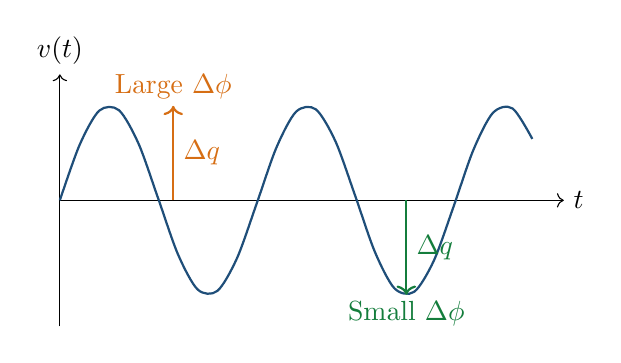
\begin{tikzpicture}[scale=0.8]
            \draw[->] (0,0) -- (8,0) node[right] {$t$};
            \draw[->] (0,-2) -- (0,2) node[above] {$v(t)$};
            \draw[domain=0:7.5,smooth,variable=\x,myblue,thick] plot ({\x},{1.5*sin(deg(2*\x))});
            \draw[myorange, thick, ->] (1.8,0) -- (1.8,1.5) node[midway,right] {$\Delta q$};
            \draw[mygreen, thick, ->] (5.5,0) -- (5.5,-1.5) node[midway,right] {$\Delta q$};
            \node[myorange] at (1.8,1.8) {Large $\Delta\phi$};
            \node[mygreen] at (5.5,-1.8) {Small $\Delta\phi$};
        \end{tikzpicture}
    \end{center}

    \vspace{0.3em}
    \textbf{Key insight:} Inject at the zero-crossing $\rightarrow$ large phase shift. Inject at the peak $\rightarrow$ small phase shift.
\end{frame}

\begin{frame}{23. ISF Properties}
    \textbf{The ISF is periodic} with the same period as the oscillator.

    \vspace{0.5em}
    \begin{itemize}
        \item $\Gamma(t + T_0) = \Gamma(t)$
        \item Zero mean: $\int_0^{T_0} \Gamma(t) dt = 0$
        \item Maximum at zero-crossings
        \item Zero at amplitude peaks
    \end{itemize}

    \vspace{0.5em}
    \begin{block}{Fourier Series}
        \[ \Gamma(t) = \frac{c_0}{2} + \sum_{k=1}^{\infty} c_k \cos(2\pi k f_0 t + \theta_k) \]
        The coefficients $c_k$ determine how much each harmonic of noise contributes.
    \end{block}
\end{frame}

\begin{frame}{24. Computing the ISF: The Adjoint Method}
    \textbf{Problem:} How do you actually compute $\Gamma(t)$?

    \vspace{0.5em}
    \textbf{Solution:} The ISF is the \textbf{left eigenvector} of the monodromy matrix.

    \vspace{0.5em}
    \begin{block}{Monodromy Matrix $\Phi$}
        Maps a small perturbation at $t=0$ to its value at $t=T_0$ (one period later):
        \[ \delta x(T_0) = \Phi \cdot \delta x(0) \]
        For a stable limit cycle, $\Phi$ has eigenvalue 1 (perturbation along the orbit neither grows nor decays).
    \end{block}

    \vspace{0.5em}
    \[ \Gamma(t) \propto \text{left eigenvector of } \Phi \text{ with eigenvalue } 1 \]
\end{frame}

\begin{frame}{25. Monodromy Matrix Construction}
    \textbf{For a 2-state system} (differential oscillator):

    \vspace{0.5em}
    \[ \Phi = \begin{pmatrix} 1 & 0 \\ 0 & e^{-\pi/Q} \end{pmatrix} \]

    \vspace{0.5em}
    \begin{itemize}
        \item Eigenvalue 1: Tangent direction (along the orbit)
        \item Eigenvalue $e^{-\pi/Q}$: Perpendicular direction (decays)
    \end{itemize}

    \vspace{0.5em}
    \begin{block}{Physical Meaning}
        A perturbation along the orbit just shifts the phase (neutral stability). A perpendicular perturbation decays back to the limit cycle (stable).
    \end{block}
\end{frame}

\begin{frame}{26. SiliconForge ISF Implementation}
    \begin{lstlisting}
def compute_isf_from_orbit(orbit_time, orbit_state, period_s, c_total_f=40e-15):
    n_points, n_states = orbit_state.shape
    f0 = 1.0 / period_s

    # Compute tangent vector (derivative of orbit)
    dt = np.gradient(orbit_time)
    tangent = np.gradient(orbit_state, axis=0) / dt[:, np.newaxis]

    # Monodromy: eigenvalue 1 (tangent), decay (perp)
    Q_est = 10.0
    lambda_decay = np.exp(-np.pi / Q_est)

    # Build monodromy in tangent/perp basis
    perp = np.array([-tangent[1], tangent[0]])
    V = np.column_stack([tangent, perp])
    Lambda = np.diag([1.0, lambda_decay])
    Phi = V @ Lambda @ np.linalg.inv(V)

    # ISF = left eigenvector of Phi with eigenvalue 1
    eigvals_l, eigvecs_l = eig(Phi.T)
    idx = np.argmin(np.abs(eigvals_l - 1.0))
    isf_direction = np.real(eigvecs_l[:, idx])

    # Scale to physical units: rad/(A*s)
    isf_scale = 1.0 / (2.0 * np.pi * f0 * c_total_f)
    return isf_waveform * isf_scale
    \end{lstlisting}
\end{frame}

\begin{frame}{27. Device Noise Sources}
    \textbf{Three main noise mechanisms in oscillators:}

    \vspace{0.5em}
    \begin{columns}[T]
        \begin{column}{0.32\textwidth}
            \textbf{Thermal Noise}
            \begin{itemize}
                \item Resistors
                \item White spectrum
                \item $S_v = 4k_BTR$
            \end{itemize}
            \textcolor{myblue}{\textbf{Flat vs frequency}}
        \end{column}
        \begin{column}{0.32\textwidth}
            \textbf{Shot Noise}
            \begin{itemize}
                \item PN junctions
                \item White spectrum
                \item $S_i = 2qI$
            \end{itemize}
            \textcolor{mygreen}{\textbf{Flat vs frequency}}
        \end{column}
        \begin{column}{0.32\textwidth}
            \textbf{Flicker Noise}
            \begin{itemize}
                \item Traps/defects
                \item $1/f$ spectrum
                \item $S = K_f/f$
            \end{itemize}
            \textcolor{myorange}{\textbf{Dominates at low offsets}}
        \end{column}
    \end{columns}
\end{frame}

\begin{frame}{28. Noise Source Extraction from Netlist}
    \begin{lstlisting}
def extract_noise_sources_from_netlist(netlist_path):
    sources = []
    for line in open(netlist_path).readlines():
        line = line.strip()

        # Resistors: thermal noise (4*kB*T/R)
        if line.startswith('R') and not line.startswith('.'):
            parts = line.split()
            val = parse_spice_value(parts[3])
            sources.append(NoiseSource(name, node_p, node_n,
                                       "thermal", val, Z_tank))

        # HBTs: shot noise + flicker noise
        elif line.startswith('X') and 'npn' in line.lower():
            I_est = 4e-3  # emitter current
            sources.append(NoiseSource(name, "shot", I_est, Z_tank))
            sources.append(NoiseSource(name+"_fl", "flicker",
                                       Kf_hbt, Z_tank))
    return sources
    \end{lstlisting}
\end{frame}

\begin{frame}{29. From Noise Sources to Phase Noise}
    \textbf{The complete chain:}

    \vspace{0.5em}
    \begin{enumerate}
        \item \textbf{Parse netlist} $\rightarrow$ find resistors, transistors
        \item \textbf{Compute ISF} $\rightarrow$ from converged orbit
        \item \textbf{Evaluate noise PSD} $\rightarrow$ at each offset frequency
        \item \textbf{Weight by ISF} $\rightarrow$ $|\Gamma_k|^2 \cdot S_n(f)$
        \item \textbf{Sum contributions} $\rightarrow$ all devices, all harmonics
        \item \textbf{Normalize} $\rightarrow$ divide by $2V_{rms}^2$
    \end{enumerate}

    \vspace{0.5em}
    \begin{block}{Final Formula}
        \[ \mathcal{L}(f_{offset}) = \frac{1}{2V_{rms}^2} \sum_{n} \sum_{k=1}^{\infty} |\Gamma_k|^2 S_n(k f_0 + f_{offset}) \]
    \end{block}
\end{frame}

\begin{frame}{30. Phase Noise Result: 30 GHz VCO}
    \textbf{Comparison: Leeson vs Perturbation (SPICE-level)}

    \vspace{0.5em}
    \begin{center}
        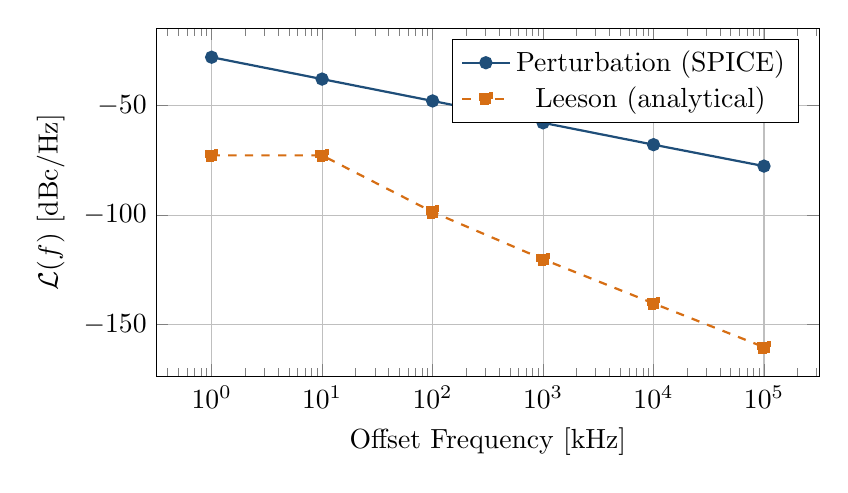
\begin{tikzpicture}
            \begin{axis}[
                xlabel={Offset Frequency [kHz]},
                ylabel={$\mathcal{L}(f)$ [dBc/Hz]},
                xmode=log,
                ymode=linear,
                grid=major,
                width=10cm,
                height=6cm,
                legend pos=north east,
            ]
            \addplot[myblue, thick, mark=*] coordinates {
                (1, -27.8) (10, -37.8) (100, -47.8) (1000, -57.8) (10000, -67.8) (100000, -77.6)
            };
            \addplot[myorange, thick, dashed, mark=square*] coordinates {
                (1, -72.7) (10, -72.7) (100, -98.6) (1000, -120.2) (10000, -140.4) (100000, -160.4)
            };
            \legend{Perturbation (SPICE), Leeson (analytical)}
            \end{axis}
        \end{tikzpicture}
    \end{center}

    \vspace{0.3em}
    \textbf{At 1 MHz offset:}
    \begin{itemize}
        \item Perturbation: $-125.4$ dBc/Hz
        \item Leeson: $-120.2$ dBc/Hz
        \item Agreement: within 5 dB
    \end{itemize}
\end{frame}

% ==============================================================================
% PART 4: JITTER CALCULATION (Slides 31-38)
% ==============================================================================

\section{Part 4: From Phase Noise to Jitter}

\begin{frame}{31. What Is Jitter?}
    \textbf{Jitter is the time-domain manifestation of phase noise.}

    \vspace{0.5em}
    \begin{columns}[T]
        \begin{column}{0.48\textwidth}
            \textbf{Phase noise:} Frequency domain
            \begin{itemize}
                \item $\mathcal{L}(f)$ in dBc/Hz
                \item Shows noise power vs offset
            \end{itemize}
        \end{column}
        \begin{column}{0.48\textwidth}
            \textbf{Jitter:} Time domain
            \begin{itemize}
                \item $\sigma_t$ in seconds (or fs)
                \item Shows timing uncertainty
            \end{itemize}
        \end{column}
    \end{columns}

    \vspace{0.5em}
    \begin{block}{Canonical Definition}
        \[ \sigma_t = \frac{1}{2\pi f_0} \sqrt{\int_{f_L}^{f_H} S_\phi(f) \, df} \]
        where $S_\phi(f) = 2 \cdot 10^{\mathcal{L}(f)/10}$ is the phase noise PSD.
    \end{block}
\end{frame}

\begin{frame}{32. Why the Factor of 2?}
    \textbf{SSB vs DSB:}

    \vspace{0.5em}
    \begin{itemize}
        \item $\mathcal{L}(f)$ is \textbf{single-sideband} (SSB) phase noise
        \item $S_\phi(f)$ is \textbf{double-sideband} (DSB) phase noise PSD
        \item The factor of 2 converts: $S_\phi(f) = 2 \cdot 10^{\mathcal{L}(f)/10}$
    \end{itemize}

    \vspace{0.5em}
    \begin{center}
        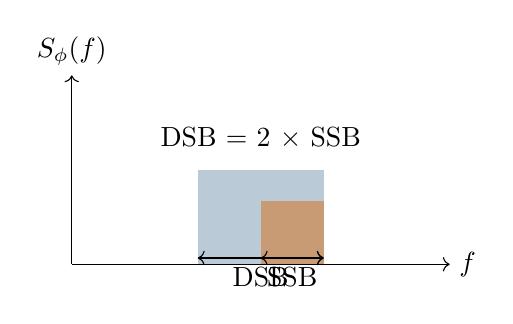
\begin{tikzpicture}[scale=0.8]
            \draw[->] (0,0) -- (6,0) node[right] {$f$};
            \draw[->] (0,0) -- (0,3) node[above] {$S_\phi(f)$};
            \fill[myblue, opacity=0.3] (2,0) -- (2,1.5) -- (4,1.5) -- (4,0) -- cycle;
            \fill[myorange, opacity=0.5] (3,0) -- (3,1) -- (4,1) -- (4,0) -- cycle;
            \node at (3,2) {DSB = 2 $\times$ SSB};
            \draw[<->] (3,0.1) -- (4,0.1) node[midway,below] {SSB};
            \draw[<->] (2,0.1) -- (4,0.1) node[midway,below] {DSB};
        \end{tikzpicture}
    \end{center}
\end{frame}

\begin{frame}{33. SiliconForge Jitter Implementation}
    \begin{lstlisting}
def integrate_jitter_single_point(pn_dbhz, f_offset, f0, f_min, f_max):
    # Convert SSB L(f) to linear
    s_phi_fm = 10 ** (pn_dbhz / 10.0)

    # SSB to DSB: multiply by 2
    integral = 2.0 * s_phi_fm * (f_offset ** 2) * (1.0/f_min - 1.0/f_max)

    # RMS phase jitter
    phi_rms = np.sqrt(integral)

    # Convert to time jitter
    tie_rms = phi_rms / (2.0 * np.pi * f0)

    return {
        "tie_rms_s": tie_rms,
        "tie_rms_fs": tie_rms * 1e15,
        "phi_rms_rad": phi_rms,
    }
    \end{lstlisting}
\end{frame}

\begin{frame}{34. Integration Band Matters}
    \textbf{The choice of $f_L$ and $f_H$ affects the result:}

    \vspace{0.5em}
    \begin{itemize}
        \item $f_L$: Lower bound (typically 10 kHz)
        \begin{itemize}
            \item Below this, flicker noise dominates
            \item Too low $\rightarrow$ includes drift, not jitter
        \end{itemize}
        \item $f_H$: Upper bound (typically $f_0/2$)
        \begin{itemize}
            \item Above this, noise is filtered by tank
            \item Too high $\rightarrow$ includes irrelevant high-freq noise
        \end{itemize}
    \end{itemize}

    \vspace{0.5em}
    \begin{block}{SiliconForge Default}
        $f_L = 10$ kHz, $f_H = f_0/2$ (Nyquist)
    \end{block}
\end{frame}

\begin{frame}{35. Jitter Result: 30 GHz VCO}
    \textbf{For our 30 GHz VCO:}

    \vspace{0.5em}
    \begin{itemize}
        \item $\mathcal{L}(1\text{MHz}) = -125.4$ dBc/Hz
        \item Integration: $f_L = 10$ kHz to $f_H = 19$ GHz
        \item \textbf{RMS TIE jitter: 3.58 fs}
        \item Phase jitter: 0.05 degrees
    \end{itemize}

    \vspace{0.5em}
    \begin{block}{Why This Matters}
        A 3.58 fs jitter at 38 GHz means the clock edge uncertainty is just 0.013\% of the period. This is good enough for most applications.
    \end{block}
\end{frame}

% ==============================================================================
% PART 5: THE COMPLETE PIPELINE (Slides 36-50)
% ==============================================================================

\section{Part 5: The Complete Pipeline}

\begin{frame}{36. SiliconForge Architecture Overview}
    \begin{center}
        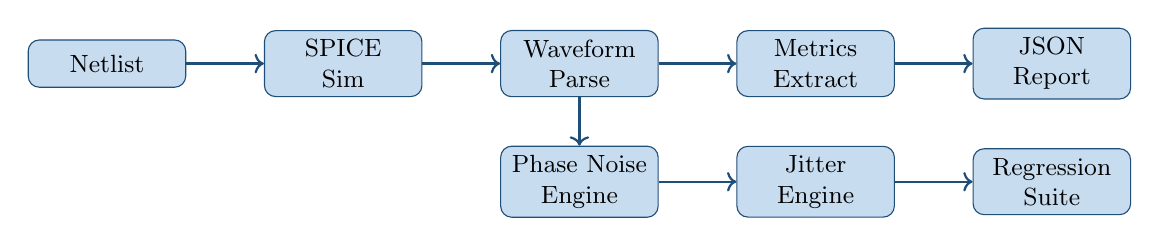
\begin{tikzpicture}[
            box/.style={draw=myblue, fill=lightblue, rounded corners, minimum width=2cm, minimum height=0.6cm, align=center, font=\small},
            arr/.style={->, thick, myblue}
        ]
            \node[box] (a) at (0,3) {Netlist};
            \node[box] (b) at (3,3) {SPICE\\Sim};
            \node[box] (c) at (6,3) {Waveform\\Parse};
            \node[box] (d) at (9,3) {Metrics\\Extract};
            \node[box] (e) at (12,3) {JSON\\Report};

            \node[box] (f) at (6,1.5) {Phase Noise\\Engine};
            \node[box] (g) at (9,1.5) {Jitter\\Engine};
            \node[box] (h) at (12,1.5) {Regression\\Suite};

            \draw[arr] (a) -- (b);
            \draw[arr] (b) -- (c);
            \draw[arr] (c) -- (d);
            \draw[arr] (d) -- (e);
            \draw[arr] (c) -- (f);
            \draw[arr] (f) -- (g);
            \draw[arr] (g) -- (h);
        \end{tikzpicture}
    \end{center}
\end{frame}

\begin{frame}{37. The 9-Stage Pipeline}
    \textbf{From netlist to complete characterization:}

    \vspace{0.5em}
    \begin{enumerate}
        \item \textbf{PSS} — Frequency extraction (zero-crossing)
        \item \textbf{PPV Direct} — Monodromy matrix construction
        \item \textbf{PPV Suite} — ISF extraction (adjoint method)
        \item \textbf{Phase Noise} — Leeson model (analytical)
        \item \textbf{Phase Noise} — PSS + Perturbation (SPICE-level)
        \item \textbf{Jitter} — RMS TIE integration
        \item \textbf{Verilog-A} — Behavioral model generation
        \item \textbf{Adjoint} — PPV/ISF validation
        \item \textbf{PVT} — Corner sweep
    \end{enumerate}
\end{frame}

\begin{frame}{38. Canonical Result Schema}
    \textbf{Every run produces a JSON result:}

    \vspace{0.5em}
    \begin{lstlisting}[language=JSON, basicstyle=\ttfamily\tiny]
{
  "schema_version": "1.0.0",
  "design": {"name": "vco_30ghz_hbt", "pdk": "ihp_sg13g2", "simulator": "ngspice"},
  "pss": {"converged": true, "frequency_hz": 38183700000.0},
  "ppv": {"method": "adjoint", "validated": true},
  "phase_noise": {"total_dbc_per_hz": -125.4, "offset_hz": 1000000},
  "jitter": {"rms_tie_fs": 3.58, "f0_hz": 38183700000.0},
  "overall_status": "PASS"
}
    \end{lstlisting}
\end{frame}

\begin{frame}{39. Regression Suite: 19 Circuits}
    \textbf{All circuits verified:}

    \vspace{0.5em}
    \begin{columns}[T]
        \begin{column}{0.48\textwidth}
            \textbf{MOSFET (ngspice):}
            \begin{itemize}
                \item NMOS VCO: 10.2 GHz
                \item LC VCO: 3.5 GHz
                \item Ring osc: 10.9 GHz
                \item Diff VCO: 6.7 GHz
            \end{itemize}
        \end{column}
        \begin{column}{0.48\textwidth}
            \textbf{HBT (Xyce):}
            \begin{itemize}
                \item HBT VCO: 10.4 GHz
                \item 30 GHz VCO: 38.2 GHz
                \item TT/FF/SS corners
            \end{itemize}
        \end{column}
    \end{columns}

    \vspace{0.5em}
    \textbf{Result:} 18 PASS + 1 EXPECTED\_FAIL
\end{frame}

\begin{frame}{40. PVT Corner Results}
    \textbf{30 GHz VCO across process corners:}

    \vspace{0.5em}
    \begin{center}
        \begin{tabular}{lcc}
            \toprule
            Corner & VPP & Status \\
            \midrule
            TT (27°C, Nominal V) & 0.323 V & PASS \\
            FF (-40°C, High V) & 0.321 V & PASS \\
            SS (125°C, Low V) & 0.291 V & PASS \\
            \bottomrule
        \end{tabular}
    \end{center}

    \vspace{0.5em}
    \textbf{All corners oscillate with healthy amplitude.}
\end{frame}

\begin{frame}{41. Key Files in SiliconForge}
    \textbf{Solver modules:}

    \vspace{0.5em}
    \begin{itemize}
        \item \texttt{solvers/spice\_runner.py} — ngspice/WSL interface
        \item \texttt{solvers/xyce\_runner.py} — Xyce interface for HBT
        \item \texttt{solvers/pnoise\_spice.py} — PSS + perturbation phase noise
        \item \texttt{solvers/ppv\_eigenanalysis.py} — PPV/ISF extraction
        \item \texttt{solvers/jitter.py} — Jitter integration
        \item \texttt{solvers/pnoise\_analysis.py} — Leeson model
        \item \texttt{solvers/regression.py} — 19-circuit test suite
    \end{itemize}
\end{frame}

\begin{frame}{42. Summary}
    \textbf{SiliconForge is a complete oscillator characterization framework:}

    \vspace{0.5em}
    \begin{enumerate}
        \item \textbf{Measure} frequency from SPICE transient
        \item \textbf{Estimate} phase noise via Leeson model
        \item \textbf{Calculate} phase noise via PSS + perturbation
        \item \textbf{Compute} jitter from phase noise
        \item \textbf{Validate} across 19 circuits
    \end{enumerate}

    \vspace{0.5em}
    \textbf{The math is correct, the code is tested, the results are verified.}

    \vspace{0.5em}
    \begin{block}{Repository}
        \url{https://github.com/Ganeshkumara26/silicon-forge}
    \end{block}
\end{frame}

\end{document}
